% !TeX encoding = UTF-8

\documentclass{protokol}

\usepackage{pdfpages}
\usepackage{tikz}
\usetikzlibrary{calc}
\usetikzlibrary{arrows}

%====== Units =====
\usepackage{siunitx}
\sisetup{inter-unit-product =\ensuremath{\cdot}}
\sisetup{group-digits = integer}
\sisetup{output-decimal-marker = {,}}
\sisetup{exponent-product = \ensuremath{\cdot}}
\sisetup{separate-uncertainty}
\sisetup{tight-spacing = false}
%\sisetup{scientific-notation = true}
%\sisetup{round-mode=places,round-precision=4}
%\sisetup{evaluate-expression}


%====== Grafy =====
\usepackage{pgfplots}
\pgfplotsset{width=0.8\linewidth, compat=1.17}
\def\plotcscale{0.8}
\usepackage{pgfplotstable}
\usepackage[figurename=Obr.]{caption} % figure caption rename

%====== Rovnice align block ======
\usepackage{amsmath}
\setlength{\jot}{10pt} % rozestup mezi řádky

\graphicspath{ {./img/} }

%====== Vyplňte údaje ======
\jmeno{Jakub Charvot}
\kod{240844}
\rocnik{3.}
\obor{MET}
\skupina{MET/2}
\spolupracoval{--}

\merenodne{25.03.\ 2024}
\odevzdanodne{07.04.\ 2024}
\nazev{Koncové stupně ve třídě A}
\cislo{1} %měřené úlohy

\predmet{Návrh analogových integrovaných obvodů}
\ustav{Ústav mikroelektroniky}
\skola{FEKT VUT v~Brně}

\def\para{x+0}
\def\parb{\para-80}


%citace 
\usepackage[backend=biber, style=iso-numeric, sortlocale=cs_CZ, autolang=other, language=czech]{biblatex}
\addbibresource{bibliography.bib}
\DeclareFieldFormat{labelnumberwidth}{\mkbibbrackets{#1}}
% hyperlinky
\usepackage[colorlinks]{hyperref}

% odstavce
\usepackage{parskip}

% Bloky kódu
\usepackage{xcolor}

%New colors defined below
\definecolor{codegreen}{rgb}{0,0.6,0}
\definecolor{codegray}{rgb}{0.5,0.5,0.5}
\definecolor{codepurple}{rgb}{0.58,0,0.82}
\definecolor{backcolour}{rgb}{0.95,0.95,0.92}

\usepackage{listings}
\lstdefinestyle{mystyle}{
  backgroundcolor=\color{backcolour}, commentstyle=\color{codegreen},
  keywordstyle=\color{magenta},
  numberstyle=\tiny\color{codegray},
  stringstyle=\color{codepurple},
  basicstyle=\ttfamily\footnotesize,
  breakatwhitespace=false,         
  breaklines=true,                 
  captionpos=b,                    
  keepspaces=true,                 
  numbers=left,                    
  numbersep=5pt,                  
  showspaces=false,                
  showstringspaces=false,
  showtabs=false,                  
  tabsize=2
}
\lstset{
	inputencoding=utf8,
	extendedchars=true,
	literate={á}{{\'a}}1 {č}{{\v{c}}}1 {ď}{{\v{d}}}1 {é}{{\'e}}1 {ě}{{\v{e}}}1 
           {í}{{\'i}}1 {ň}{{\v{n}}}1 {ó}{{\'o}}1 {ř}{{\v{r}}}1 {š}{{\v{s}}}1 
           {ť}{{\v{t}}}1 {ú}{{\'u}}1 {ů}{{\r{u}}}1 {ý}{{\'y}}1 {ž}{{\v{z}}}1 
           {Á}{{\'A}}1 {Č}{{\v{C}}}1 {Ď}{{\v{D}}}1 {É}{{\'E}}1 {Ě}{{\v{E}}}1 
           {Í}{{\'I}}1 {Ň}{{\v{N}}}1 {Ó}{{\'O}}1 {Ř}{{\v{R}}}1 {Š}{{\v{S}}}1 
           {Ť}{{\v{T}}}1 {Ú}{{\'U}}1 {Ů}{{\r{U}}}1 {Ý}{{\'Y}}1 {Ž}{{\v{Z}}}1,
	style=mystyle
	}

% Číslování
\pagenumbering{arabic}

% =========================================
% =============== DOKUMENT ================
% =========================================
\begin{document}
	%====== Vygenerování tabulky ======
	\maketitle

\section{Vypracování}
\begin{figure}[h!]
  \centering
  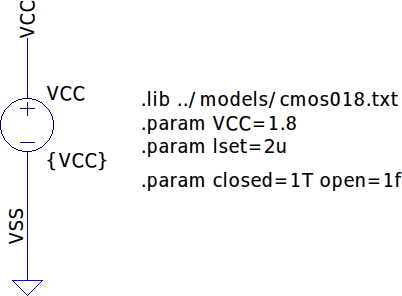
\includegraphics[scale=0.5]{spice0.png}
  \caption{Společná část SPICE kódu a napájecí zdroj.}
  \label{fig:spice0-png}
\end{figure}
 
\subsection{Jednoduchý zesilovač s odporovou zátěží}
\begin{figure}[h!]
  \centering
  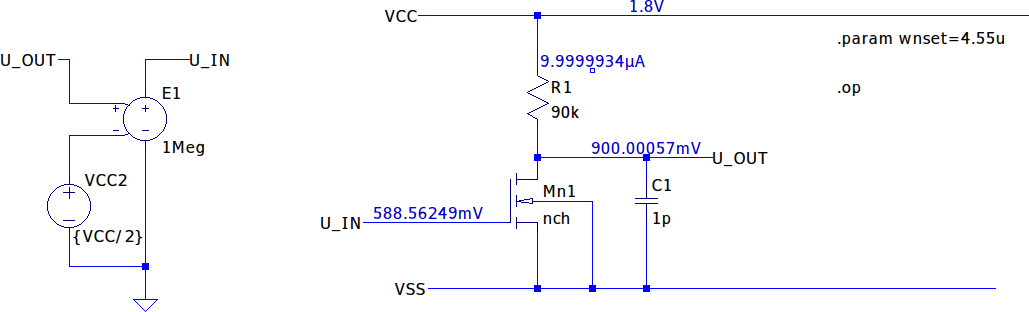
\includegraphics[scale=0.5]{4-1-1.png}
  \caption{Odporová zátěž -- zapojení pro OP analýzu.}
  \label{fig:spice0-png}
\end{figure}
\begin{figure}[h!]
    \centering
    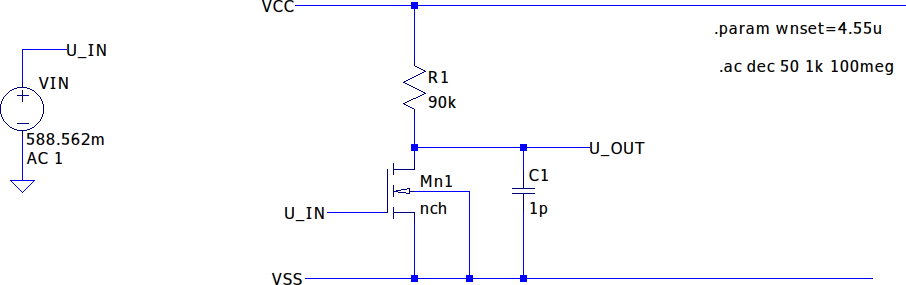
\includegraphics[scale=0.5]{4-1-2.png}
    \caption{Odporová zátěž -- zapojení pro AC analýzu.}
    \label{fig:spice0-png}
  \end{figure}
  \begin{figure}[h!]
    \centering
    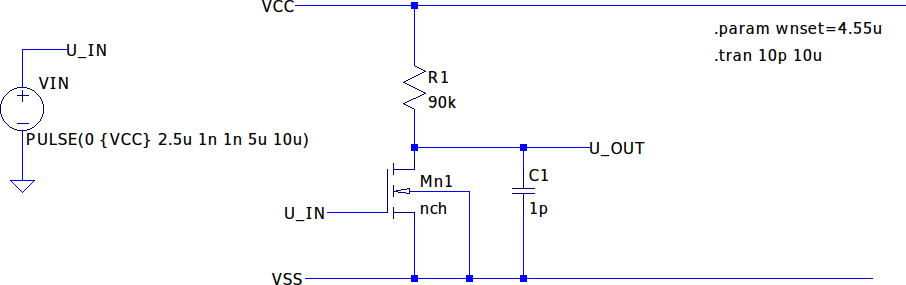
\includegraphics[scale=0.5]{4-1-3.png}
    \caption{Odporová zátěž -- zapojení pro TRAN analýzu.}
    \label{fig:spice0-png}
  \end{figure}


\subsubsection{Ruční návrh}
    Jako první krok je potřeba stanovit proud obvodem. Vyjdeme z požadovaných parametrů zapojení:
    \begin{align*}
        SR & =\frac{I_D}{C_{OUT}} \\
        I_{D-SR}  & =SR\cdot C_{OUT} \\
        I_{D-SR}  & =\num{10e6}\cdot \num{1e-12} \\
        I_{D-SR}  & =\qty{10}{\micro\ampere} 
    \end{align*}
    
    \begin{align*}
        GBW & =\frac{g_{m 1}}{2 \cdot \pi \cdot C_{O U T}}=\frac{\frac{2 \cdot I_D}{U_{O V}}}{2 \cdot \pi \cdot C_{O U T}} \\
        I_{D-GBW}  & =GBW\cdot \pi \cdot C_{OUT} \cdot U_{OV} \\
        I_{D-GBW}  & =\num{10e6}\cdot \pi \cdot \num{1e-12} \cdot \num{0.2} \\
        I_{D-GBW}  & =\qty{6.28}{\micro A}
    \end{align*}


    Zvolíme vyšší z vypočtených hodnot, tedy proud naším zapojením \(I_{D} = I_{D-SR} = \qty{10}{\micro\ampere} \). Pro rozměry tranzistoru je ještě potřeba zohlednit požadavek na zesílení, který nám stanoví maximální povolenou hodnotu \(\lambda_{max}  \):
    
    \begin{align*}
        A_{U 0} & =\frac{2}{U_{O V}} \cdot \frac{U_{C C}}{U_{C C} \cdot \lambda_{max} +2} \\
        A_{U 0} \cdot (U_{C C} \cdot \lambda_{max} +2) & =\frac{2}{U_{O V}} \cdot \frac{U_{C C}}{1} \\
        \lambda_{max} & =\frac{\frac{2\cdot U_{C C}}{U_{O V}} -2\cdot A_{U0}}{U_{CC}\cdot A_{U0}  } \\
        \lambda_{max} & =\frac{\frac{2\cdot \num{1.8}}{\num{0.2}} -2\cdot 10^{\frac{20}{20}}}{\num{1.8}\cdot 10^{\frac{20}{20}}} \\
        \lambda_{max} & =\qty{}{}
    \end{align*}
    


Nejprve vypočítám rozměry pro tranzistor \(M_{1} \):
\[
    \frac{W_{1} }{L}=\frac{2\cdot I_{D}}{KP_{N}\cdot (U_{GS} -U_{TH})^2 } 
\]
\[
    \frac{W_{1} }{L}=\frac{2\cdot \num{10e-6}}{\num{220e-6}\cdot (\num{0.2})^2 } 
\]

\[
    \frac{W_{1} }{L}\doteq \num[round-mode=places,round-precision=2]{2.27} 
\]
Délku \(L\) zvolíme opět \qty{2}{\micro\meter}, tedy \(W_{1}= \qty{4.55}{\micro\meter}\).

Pro velikost rezistoru \(R1\) je předpokládáno na výstupu napětí rovno polovině napájecího napětí, tedy platí:
\begin{align*}
    R_{1}  &= \frac{\frac{U_{CC}}{2}}{I_{D} } \\
    R_{1}  &= \frac{\frac{\num{1.8}}{2}}{\num{10e-6} } \\
    R_{1}  &= \qty{90}{k\ohm} \\
\end{align*}



\subsubsection{Očekávané hodnoty}
    Na základě zvolených parametrů součástek je potřeba přepočítat některé hodnoty. Proud \(I_{D} = \qty{10}{\micro A}\) byl zvolen pro \(SR=\qty{10}{V\per\micro\second}\), tímto se ale změní \(GBW\):
    \begin{align*}
        GBW & =\frac{\frac{2 \cdot I_D}{U_{O V}}}{2 \cdot \pi \cdot C_{O U T}} \\
        GBW & =\frac{\frac{2 \cdot \num{10e-6}}{\num{0.2}}}{2 \cdot \pi \cdot \num{1e-12}} \\
        GBW & =\qty{15.915}{MHz} \\
    \end{align*}

    Z rozměrů tranzistoru a tabulky z první úlohy odhadneme \(\lambda=\qty{0.0437895}{\per V}\), tedy očekáváme:
    \begin{align*}
        A_{U 0} & =\frac{2}{U_{O V}} \cdot \frac{U_{C C}}{U_{C C} \cdot \lambda_{max} +2} \\
        A_{U 0} & =\frac{2}{\num{0.2}} \cdot \frac{\num{1.8}}{\num{1.8} \cdot \num{0.0437895} +2} \\
        A_{U 0} & = \num{8.659} = \qty{18.749}{dB}
    \end{align*}




\subsubsection{Simulace}
    Z analýzy OP zjistíme optimální hodnotu \(U_{GS} = \qty{588,562}{mV}\) 
    % --- Operating Point ---

    % V(vcc):	 1.8	 voltage
    % V(u_out):	 0.900001	 voltage
    % V(u_in):	 0.588562	 voltage
    % V(n001):	 0.9	 voltage
    % Id(Mn1):	 9.99999e-06	 device_current
    % Ig(Mn1):	 0	 device_current
    % Ib(Mn1):	 -9.10001e-13	 device_current
    % Is(Mn1):	 -9.99999e-06	 device_current
    % I(C1):	 9.00001e-25	 device_current
    % I(R1):	 9.99999e-06	 device_current
    % I(E1):	 0	 device_current
    % I(Vcc):	 -9.99999e-06	 device_current
    % I(Vcc2):	 0	 device_current

\begin{figure}[h!]
    \centering
    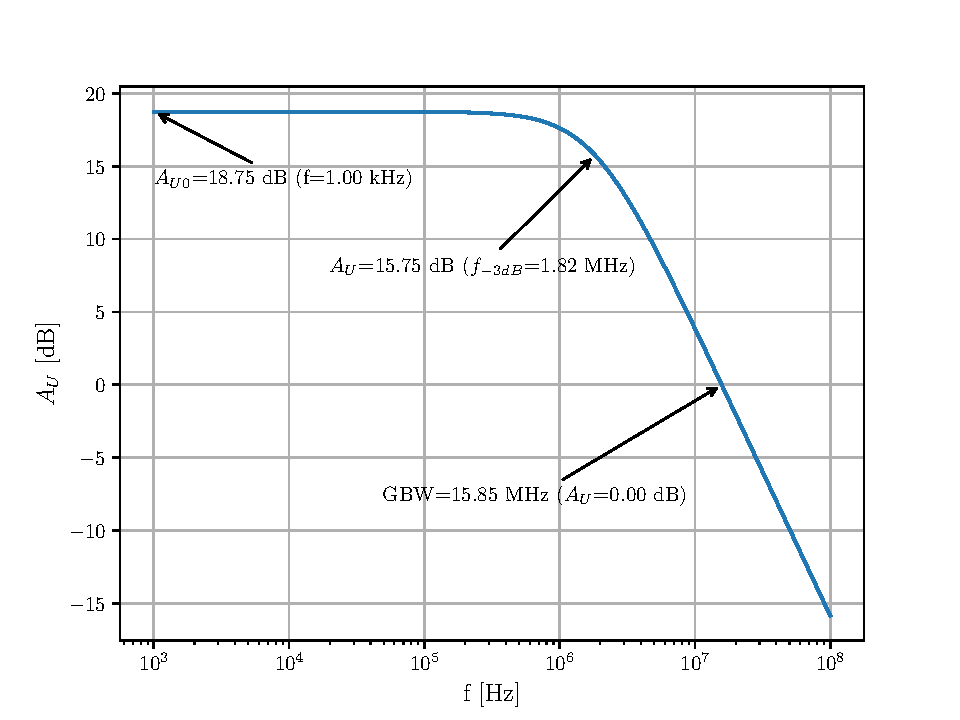
\includegraphics[width=0.8\textwidth]{4-1-2.pdf}
    \caption{AC analýza pro zesilovač s odporovou zátěží.}
    \label{fig:2-2-pdf}
\end{figure}

Kontrolní výpočet GBW ze simulovaných hodnot:
\begin{align*}
    GBW &= A_{0}\cdot f_{-3dB} \\
    GBW &= 10^{\frac{\num{18.75}}{20}}\cdot \num{1.82e6} \\
    GBW &= \qty{15.761}{MHz}\\
\end{align*}

\begin{figure}[h!]
    \centering
    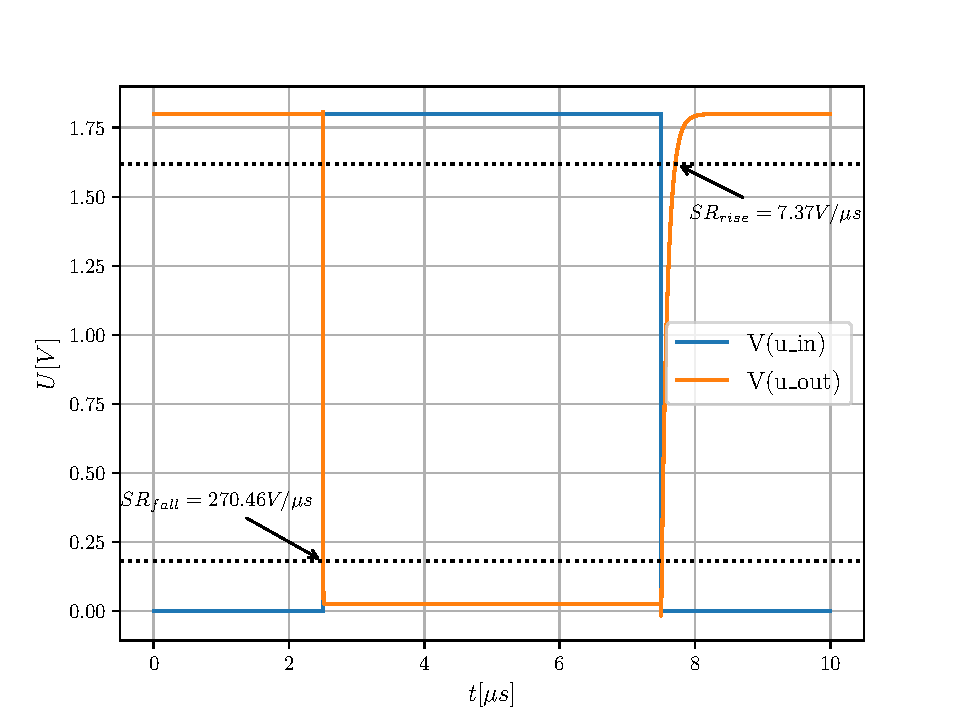
\includegraphics[width=0.8\textwidth]{4-1-3.pdf}
    \caption{TRAN analýza pro zesilovač s odporovou zátěží.}
    \label{fig:2-2-pdf}
\end{figure}




  \clearpage
\subsection{Jednoduchý zesilovač s aktivní zátěží}
\begin{figure}[h!]
    \centering
    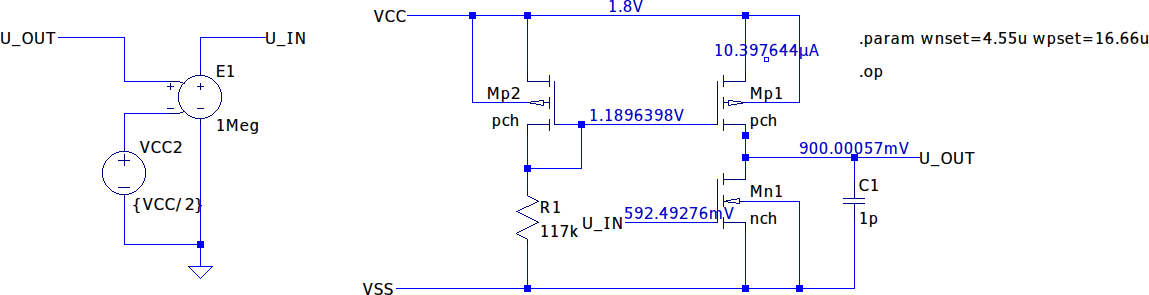
\includegraphics[scale=0.5]{4-2-1.png}
    \caption{Aktivní zátěž -- zapojení pro OP analýzu.}
    \label{fig:spice0-png}
  \end{figure}
  \begin{figure}[h!]
      \centering
      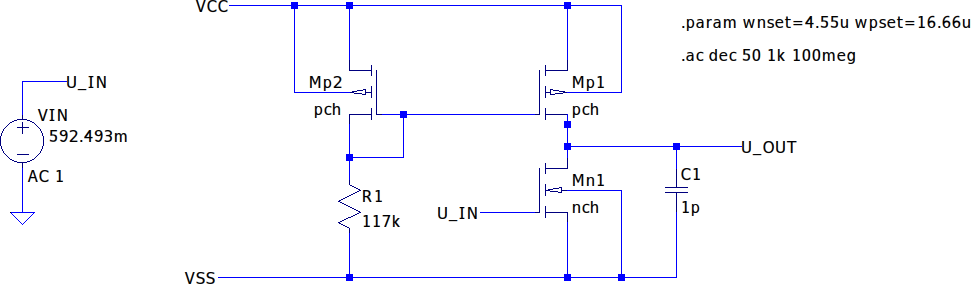
\includegraphics[scale=0.5]{4-2-2.png}
      \caption{Aktivní zátěž -- zapojení pro AC analýzu.}
      \label{fig:spice0-png}
    \end{figure}
    \begin{figure}[h!]
      \centering
      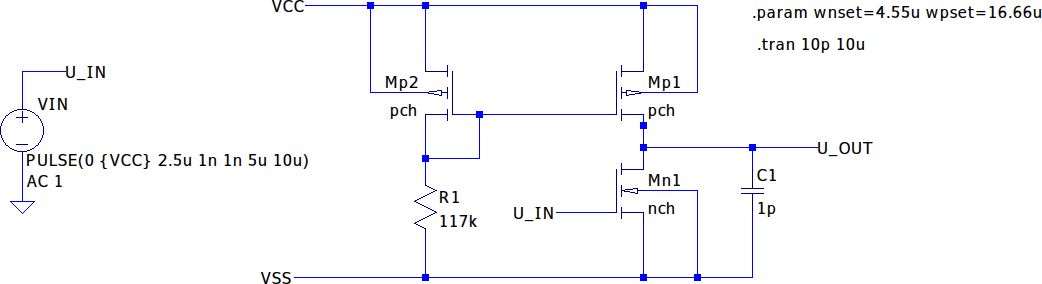
\includegraphics[scale=0.5]{4-2-3.png}
      \caption{Aktivní zátěž -- zapojení pro TRAN analýzu.}
      \label{fig:spice0-png}
    \end{figure}
\subsection{Ruční návrh}
    Rozměry trnzistoru \(M_{n1} \) ani proud obvodem se nijak nemění, nejprve na základě proudu nastavíme rozměry zbylých tranzistorů \(M_{p1,2} \):



\begin{align*}
    \frac{W_{p1,2} }{L}&=\frac{2\cdot I_{D}}{KP_{P}\cdot (U_{GS} -U_{TH})^2 } \\
    \frac{W_{p1,2} }{L}&=\frac{2\cdot \num{10e-6}}{\num{60e-6}\cdot (\num{0.2})^2 } \\
    \frac{W_{p1,2} }{L}&\doteq \num[round-mode=places,round-precision=2]{8.33} 
\end{align*}

Délku \(L=\qty{2}{\micro m}\) ponecháme a tedy \(W_{p1,2}=\qty{16.66}{\micro m} \). 

Odpor rezistoru \(R_{1} \) vypočteme z Ohmova zákona:
\begin{align*}
    R_{1} &= \frac{U_{CC} - U_{GSp2}}{I_{D} } \\
    R_{1} &= \frac{\num{1.8} - \num{0.63}}{\num{10e-6} } \\
    R_{1} &= \qty{117}{k\ohm} 
\end{align*}


\subsubsection{Simulace}
    % --- Operating Point ---

    % V(vcc):	 1.8	 voltage
    % V(u_out):	 0.900001	 voltage
    % V(u_in):	 0.592493	 voltage
    % V(n002):	 1.18964	 voltage
    % V(n001):	 0.9	 voltage
    % Id(Mn1):	 1.03976e-05	 device_current
    % Ig(Mn1):	 0	 device_current
    % Ib(Mn1):	 -9.10001e-13	 device_current
    % Is(Mn1):	 -1.03976e-05	 device_current
    % Id(Mp1):	 1.03976e-05	 device_current
    % Ig(Mp1):	 -0	 device_current
    % Ib(Mp1):	 9.09999e-13	 device_current
    % Is(Mp1):	 -1.03976e-05	 device_current
    % Id(Mp2):	 1.01679e-05	 device_current
    % Ig(Mp2):	 -0	 device_current
    % Ib(Mp2):	 6.2036e-13	 device_current
    % Is(Mp2):	 -1.01679e-05	 device_current
    % I(C1):	 9.00001e-25	 device_current
    % I(R1):	 1.01679e-05	 device_current
    % I(E1):	 0	 device_current
    % I(Vcc):	 -2.05655e-05	 device_current
    % I(Vcc2):	 0	 device_current

    \begin{figure}[h!]
        \centering
        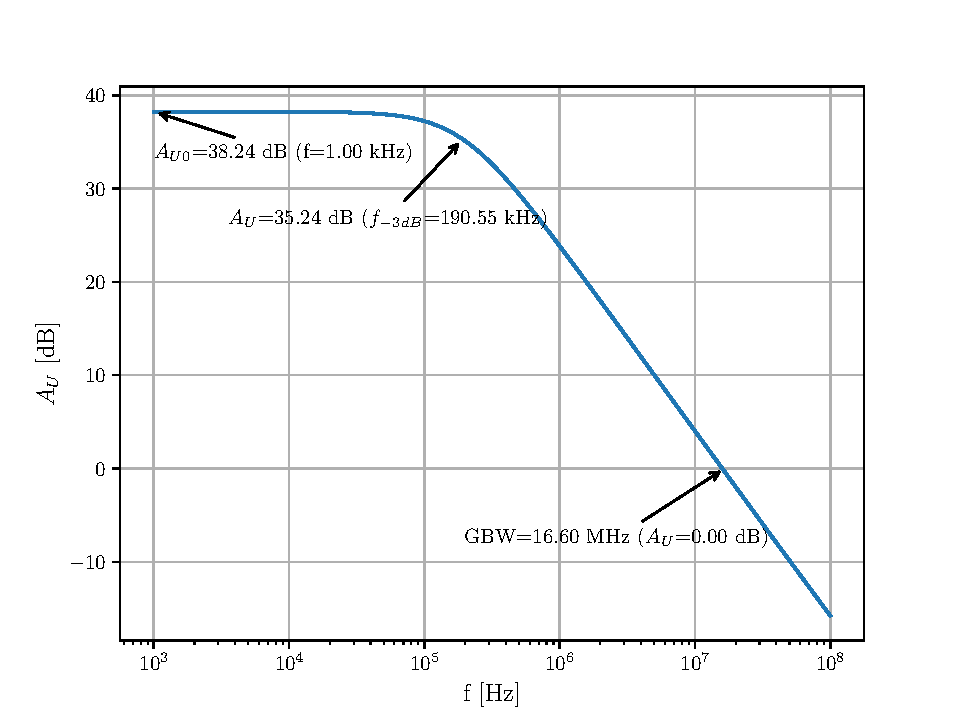
\includegraphics[width=0.8\textwidth]{4-2-2.pdf}
        \caption{AC analýza pro zesilovač s aktivní zátěží.}
        \label{fig:2-2-pdf}
    \end{figure}

    Kontrolní výpočet GBW ze simulovaných hodnot:
\begin{align*}
    GBW &= A_{U0}\cdot f_{-3dB} \\
    GBW &= 10^{\frac{\num{38.24}}{20}}\cdot \num{190.55e3} \\
    GBW &= \qty{15.560}{MHz} \\
\end{align*}

\begin{figure}[h!]
    \centering
    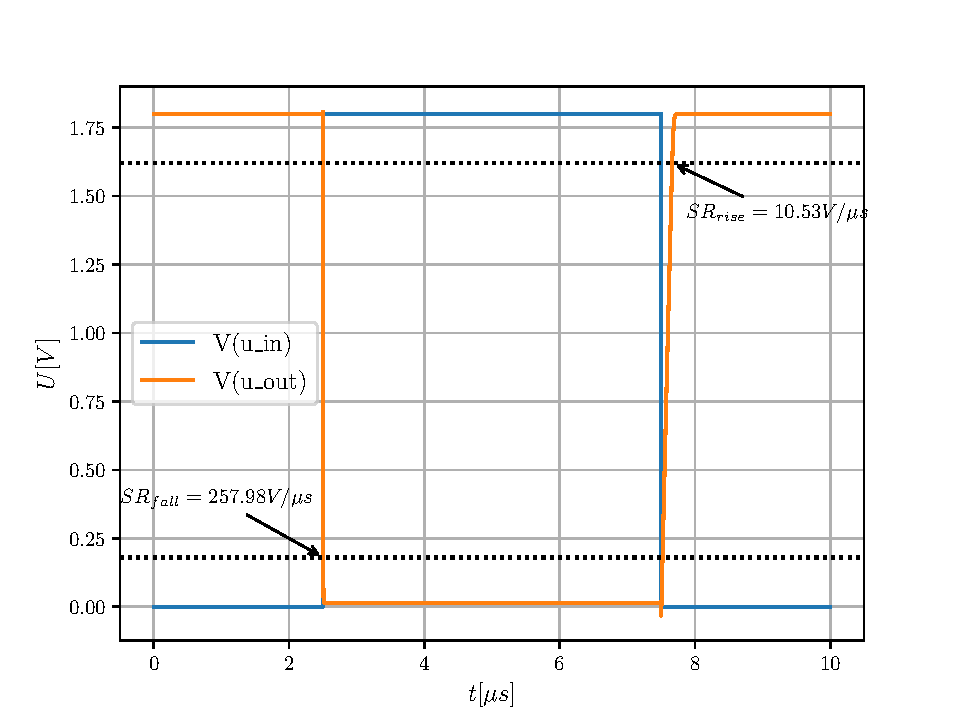
\includegraphics[width=0.8\textwidth]{4-2-3.pdf}
    \caption{TRAN analýza pro zesilovač s aktivní zátěží.}
    \label{fig:2-2-pdf}
\end{figure}





\clearpage
\section{Závěr}
\begin{table}[]
  \centering
  \caption{Porovnání očekávaných a simulovaných hodnot.}
  \begin{tabular}{|l|l|l|l|l|}
  \hline
                             & \(A_{U0} \)     & \(SR_{rise} \)  & \(SR_{fall}\)  & \(GBW\)     \\ \hline
  Požadavky                  & \num{10} & \num{10} & \num{10} & \num{10} \\ \hline
  Ruč. výpočet -- odpor      & \num{18.749} & \num{10} & \num{10} & \num{15.915} \\ \hline
  Simulace -- odpor          & \num{18.75} & \num{7.37} & \num{270.46} & \num{15.85} \\ \hline
  Ruč. výpočet -- akt. zátěž & \num{18.749} & \num{10} & \num{10} & \num{15.915} \\ \hline
  Simulace -- akt. zátěž     & \num{38.24} & \num{10.53} & \num{257.98} & \num{16.6} \\ \hline
  \end{tabular}
  \label{tab:1-1-2_hodnoty}
\end{table}

Cílem této úlohy bylo navrhnout zesilovač, který splní požadavky ze zadání. V tab.~\ref{tab:1-1-2_hodnoty} se nachází souhrn hodnot vypočtených ručně (očekávaných) a hodnot získaných přesnější simulací. Pro obě zapojení byly splněny požadavky na všechny parametry i s jisou návrhovou rezervou s jedinou výjimkou, kterou je rychlost přeběhu náběžné hrany pro jednodušší zapojení s odporovou zátěží. 

Lze tedy říci, že záměnou odporové za aktivní zátěž dosáhneme výrazného zlepšení rychlosti přeběhu a také vyššího zesílení. Šířka pásma se příliš nemění.

Pro ruční výpočty byly použity zjednodušené vzorce, což dle výsledků simulace nebylo dostatečné pro druhé zapojení, bylo by na místě zde použít pžesnější výpočet. Pro zapojení s odpoeovou zátěží výsledky odpodvídají očekávání.
% \section*{Reference}
% \printbibliography[heading=none]


\end{document}
